\section{Definição}

\begin{frame}[fragile]{Definição de heap binária}

    \begin{itemize}
        \item A \textit{heap} binária é uma estrutura de dados que mantém um conjunto de elementos,
            organizados de forma a permitir a identificação eficiente do menor
            dentro todos estes elementos

        \item Uma variante comum da \textit{heap} binária é a troca da identificação do menor
            elemento para a identificação do maior dentre seus elementos

        \item As duas operações principais de uma \textit{heap} binária são a inserção de novos
            elementos ou a identificação (e extração) do menor elemento

        \item Outra operação importante é a construção de uma
            \textit{heap} a partir de uma sequência de elementos dados
    \end{itemize}

\end{frame}

\begin{frame}[fragile]{Propriedade fundamental de uma \textit{heap} binária}

    \begin{itemize}
        \item Uma \textit{heap} binária pode ser implementada a partir de uma árvore binária
            ou de um vetor

        \item A primeira alternativa tem como vantagem a visualização mais natural da 
            propriedade fundamental das \textit{heaps}

        \item A segunda permite uma implementação eficiente em termos de memória
    \end{itemize}

    \metroset{block=fill}
    \begin{block}{Propriedade fundamental da \textit{heap} binária}
        Para qualquer elemento $x$ contido na \textit{heap}, a chave de $x$ é menor ou igual  do
        que as chaves de todos os seus descendentes.
    \end{block}
	
\end{frame}

\begin{frame}[fragile]{Heaps como árvores}

    \begin{itemize}
        \item A visualização de uma \textit{heap} como uma árvore binária permite a 
            identificação de propriedades consequentes da propriedade fundamental

        \item Primeiramente, a raiz da árvore será o menor dentre todos os elementos

        \item Em segundo lugar, a representação da \textit{heap} não é única

        \item Além disso, a travessia de uma folha até a raiz leva a um caminho cujas chaves
            estão em ordem decrescente

        \item Esta propriedade é fundamental para a implementação das operações de inserção e
            remoção de elementos de um elemento
    \end{itemize}

\end{frame}

% Sequência de inserção: 40, 98, 17, 33, 21, 57, 40, 89, 62, 74
\begin{frame}[fragile]{Exemplo de {\it max heap} binária}

    \begin{figure}
        \centering
        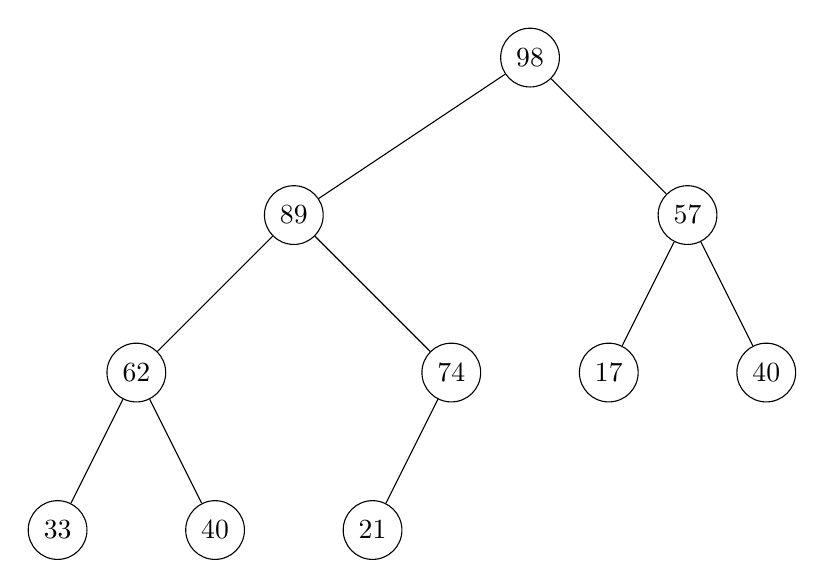
\begin{tikzpicture}
                \node[circle,draw] (A) at (6, 6) { 98 };
                \node[circle,draw] (B) at (3, 4) { 89 };
                \node[circle,draw] (C) at (8, 4) { 57 };
                \node[circle,draw] (D) at (1, 2) { 62 };
                \node[circle,draw] (E) at (5, 2) { 74 };
                \node[circle,draw] (F) at (7, 2) { 17 };
                \node[circle,draw] (G) at (9, 2) { 40 };
                \node[circle,draw] (H) at (0, 0) { 33 };
                \node[circle,draw] (I) at (2, 0) { 40 };
                \node[circle,draw] (J) at (4, 0) { 21 };

                \draw (A) -- (B);
                \draw (A) -- (C);
                \draw (B) -- (D);
                \draw (B) -- (E);
                \draw (C) -- (F);
                \draw (C) -- (G);
                \draw (D) -- (H);
                \draw (D) -- (I);
                \draw (E) -- (J);
        \end{tikzpicture}
    \end{figure}

\end{frame}

\begin{frame}[fragile]{\textit{Heaps} binárias como vetores}

    \begin{itemize}
        \item Uma \textit{heap} binária pode ser armazenada como uma árvore balanceada

        \item Esta propriedade permite o armazenamento de seus elementos em um vetor

        \item Se a raiz for armazenada no índice 1 (e não no zero), as relações de parentesco
            ficam simplificadas, através de operações simples

        \item O pai de um elemento $x$ que ocupa o índice $i$ está localizado no índice 
            $p = \lfloor i/2\rfloor$

        \item O filho à esquerda de $x$ tem índice $l = 2i$
        \item O filho à direita  de $x$ tem índice $r = 2i + 1$

        \item Mesmo que o índice zero fique inutilizado, a economia de memória em relação à 
            representação com árvore é notável: como os parentes podem ser localizados a partir
            de seus índices, não é necessário armazenar ponteiros

        \item Observe a relação entre a representação como vetor e uma travessia em largura
            da árvore binária
    \end{itemize}

\end{frame}

\begin{frame}[fragile]{Visualização de uma heap binária como árvore e como vetor}

    \begin{figure}
        \centering
        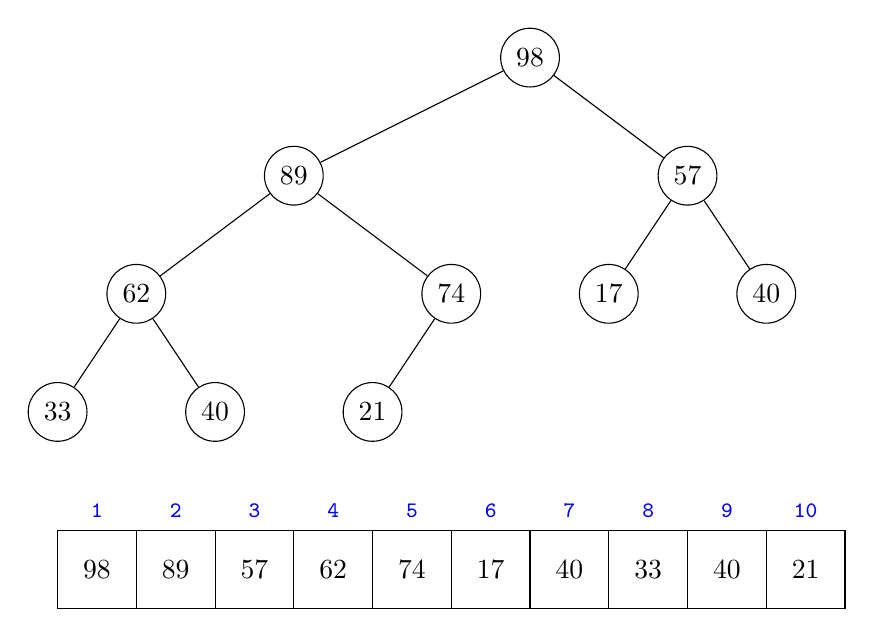
\begin{tikzpicture}
                \node[circle,draw] (A) at (6, 6) { 98 };
                \node[circle,draw] (B) at (3, 4.5) { 89 };
                \node[circle,draw] (C) at (8, 4.5) { 57 };
                \node[circle,draw] (D) at (1, 3) { 62 };
                \node[circle,draw] (E) at (5, 3) { 74 };
                \node[circle,draw] (F) at (7, 3) { 17 };
                \node[circle,draw] (G) at (9, 3) { 40 };
                \node[circle,draw] (H) at (0, 1.5) { 33 };
                \node[circle,draw] (I) at (2, 1.5) { 40 };
                \node[circle,draw] (J) at (4, 1.5) { 21 };

                \draw (A) -- (B);
                \draw (A) -- (C);
                \draw (B) -- (D);
                \draw (B) -- (E);
                \draw (C) -- (F);
                \draw (C) -- (G);
                \draw (D) -- (H);
                \draw (D) -- (I);
                \draw (E) -- (J);

                \draw (0, -1) grid (10, 0);

                \node[color=blue] at (0.5, 0.25) { \footnotesize \texttt{\textbf{1}} };
                \node[color=blue] at (1.5, 0.25) { \footnotesize \texttt{\textbf{2}} };
                \node[color=blue] at (2.5, 0.25) { \footnotesize \texttt{\textbf{3}} };
                \node[color=blue] at (3.5, 0.25) { \footnotesize \texttt{\textbf{4}} };
                \node[color=blue] at (4.5, 0.25) { \footnotesize \texttt{\textbf{5}} };
                \node[color=blue] at (5.5, 0.25) { \footnotesize \texttt{\textbf{6}} };
                \node[color=blue] at (6.5, 0.25) { \footnotesize \texttt{\textbf{7}} };
                \node[color=blue] at (7.5, 0.25) { \footnotesize \texttt{\textbf{8}} };
                \node[color=blue] at (8.5, 0.25) { \footnotesize \texttt{\textbf{9}} };
                \node[color=blue] at (9.5, 0.25) { \footnotesize \texttt{\textbf{10}} };

                \node at (0.5, -0.5) { 98 };
                \node at (1.5, -0.5) { 89 };
                \node at (2.5, -0.5) { 57 };
                \node at (3.5, -0.5) { 62 };
                \node at (4.5, -0.5) { 74 };
                \node at (5.5, -0.5) { 17 };
                \node at (6.5, -0.5) { 40 };
                \node at (7.5, -0.5) { 33 };
                \node at (8.5, -0.5) { 40 };
                \node at (9.5, -0.5) { 21 };
        \end{tikzpicture}
    \end{figure}

\end{frame}

\begin{frame}[fragile]{Exemplo de implementação de uma heap usando vector}
    \inputsnippet{cpp}{1}{19}{codes/heap.cpp}
\end{frame}
